\chapter{Matrice}

\index{matrica}

\key{Matrica} je matematički pojam
koji odgovara dvodimenzionalnom nizu
u programiranju. Na primjer,
\[
A = 
 \begin{bmatrix}
  6 & 13 & 7 & 4 \\
  7 & 0 & 8 & 2 \\
  9 & 5 & 4 & 18 \\
 \end{bmatrix}
\]
je matrica veličine $3 \times 4$, tj.
ima 3 reda i 4 stupca.
Oznaka $[i,j]$ odnosi se na
element u retku $i$ i stupcu $j$
matrice.
Na primjer, u gornjoj matrici vrijedi
$A[2,3]=8$ i $A[3,1]=9$.

\index{vektor}

Poseban slučaj matrice je \key{vektor},
odnosno jednodimenzionalna matrica veličine $n \times 1$.
Na primjer,
\[
V =
\begin{bmatrix}
4 \\
7 \\
5 \\
\end{bmatrix}
\]
je vektor koji sadrži tri elementa.

\index{transponirana matrica}

\key{Transponirana matrica} $A^T$ matrice $A$
dobiva se zamjenom redaka i stupaca matrice $A$,
tj. $A^T[i,j]=A[j,i]$:
\[
A^T = 
 \begin{bmatrix}
  6 & 7 & 9 \\
  13 & 0 & 5 \\
  7 & 8 & 4 \\
  4 & 2 & 18 \\
 \end{bmatrix}
\]

\index{kvadratna matrica}

Matrica je \key{kvadratna matrica} ako
ima jednak broj redaka i stupaca.
Na primjer, sljedeća matrica je
kvadratna matrica:

\[
S = 
 \begin{bmatrix}
  3 & 12 & 4  \\
  5 & 9 & 15  \\
  0 & 2 & 4 \\
 \end{bmatrix}
\]

\section{Operacije}

Zbroj $A+B$ matrica $A$ i $B$
definiran je ako su matrice jednakih veličina.
Rezultat je matrica u kojoj je svaki element
zbroj odgovarajućih elemenata
matrica $A$ i $B$.

Na primjer,
\[
 \begin{bmatrix}
  6 & 1 & 4 \\
  3 & 9 & 2 \\
 \end{bmatrix}
+
 \begin{bmatrix}
  4 & 9 & 3 \\
  8 & 1 & 3 \\
 \end{bmatrix}
=
 \begin{bmatrix}
  6+4 & 1+9 & 4+3 \\
  3+8 & 9+1 & 2+3 \\
 \end{bmatrix}
=
 \begin{bmatrix}
  10 & 10 & 7 \\
  11 & 10 & 5 \\
 \end{bmatrix}.
\]

Množenje matrice $A$ vrijednošću $x$ znači
da se svaki element matrice $A$ množi s $x$.
Na primjer,
\[
 2 \cdot \begin{bmatrix}
  6 & 1 & 4 \\
  3 & 9 & 2 \\
 \end{bmatrix}
=
 \begin{bmatrix}
  2 \cdot 6 & 2\cdot1 & 2\cdot4 \\
  2\cdot3 & 2\cdot9 & 2\cdot2 \\
 \end{bmatrix}
=
 \begin{bmatrix}
  12 & 2 & 8 \\
  6 & 18 & 4 \\
 \end{bmatrix}.
\]

\subsubsection{Množenje matrica}

\index{množenje matrica}

Umnožak $AB$ matrica $A$ i $B$
definiran je ako je $A$ veličine $a \times n$,
a $B$ veličine $n \times b$, tj.
ako je širina matrice $A$ jednaka visini matrice $B$.
Rezultat je matrica veličine $a \times b$
čiji se elementi računaju formulom
\[
AB[i,j] = \sum_{k=1}^n A[i,k] \cdot B[k,j].
\]

Ideja je da je svaki element matrice $AB$
suma umnožaka elemenata matrica $A$ i $B$
prema sljedećoj slici:

\begin{center}
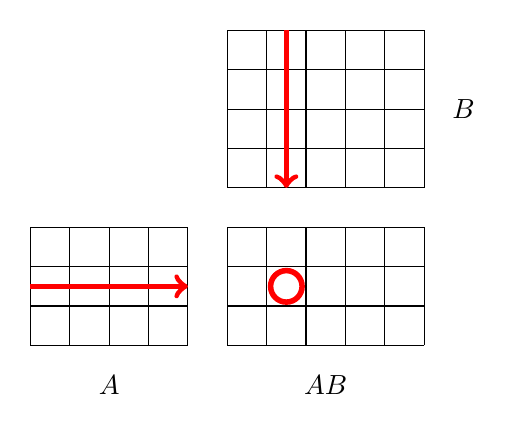
\begin{tikzpicture}[scale=0.5]
\draw (0,0) grid (4,3);
\draw (5,0) grid (10,3);
\draw (5,4) grid (10,8);

\node at (2,-1) {$A$};
\node at (7.5,-1) {$AB$};
\node at (11,6) {$B$};

\draw[thick,->,red,line width=2pt] (0,1.5) -- (4,1.5);
\draw[thick,->,red,line width=2pt] (6.5,8) -- (6.5,4);
\draw[thick,red,line width=2pt] (6.5,1.5) circle (0.4);
\end{tikzpicture}
\end{center}

Na primjer,

\[
 \begin{bmatrix}
  1 & 4 \\
  3 & 9 \\
  8 & 6 \\
 \end{bmatrix}
\cdot
 \begin{bmatrix}
  1 & 6 \\
  2 & 9 \\
 \end{bmatrix}
=
 \begin{bmatrix}
  1 \cdot 1 + 4 \cdot 2 & 1 \cdot 6 + 4 \cdot 9 \\
  3 \cdot 1 + 9 \cdot 2 & 3 \cdot 6 + 9 \cdot 9 \\
  8 \cdot 1 + 6 \cdot 2 & 8 \cdot 6 + 6 \cdot 9 \\
 \end{bmatrix}
=
 \begin{bmatrix}
  9 & 42 \\
  21 & 99 \\
  20 & 102 \\
 \end{bmatrix}.
\]

Množenje matrica je asocijativno,
pa vrijedi $A(BC)=(AB)C$,
ali nije komutativno,
pa $AB = BA$ obično ne vrijedi.

\index{jedinična matrica}

\key{Jedinična matrica} je kvadratna matrica
u kojoj je svaki element na dijagonali jednak 1,
a svi ostali elementi jednaki 0.
Na primjer, sljedeća matrica
je jedinična matrica veličine $3 \times 3$:
\[
 I = \begin{bmatrix}
  1 & 0 & 0 \\
  0 & 1 & 0 \\
  0 & 0 & 1 \\
 \end{bmatrix}
\]

\begin{samepage}
Množenje matrice jediničnom matricom
ne mijenja je. Na primjer,
\[
 \begin{bmatrix}
  1 & 0 & 0 \\
  0 & 1 & 0 \\
  0 & 0 & 1 \\
 \end{bmatrix}
\cdot
 \begin{bmatrix}
  1 & 4 \\
  3 & 9 \\
  8 & 6 \\
 \end{bmatrix}
=
 \begin{bmatrix}
  1 & 4 \\
  3 & 9 \\
  8 & 6 \\
 \end{bmatrix} \hspace{10px} \textrm{i} \hspace{10px}
 \begin{bmatrix}
  1 & 4 \\
  3 & 9 \\
  8 & 6 \\
 \end{bmatrix}
\cdot
 \begin{bmatrix}
  1 & 0 \\
  0 & 1 \\
 \end{bmatrix}
=
 \begin{bmatrix}
  1 & 4 \\
  3 & 9 \\
  8 & 6 \\
 \end{bmatrix}.
\]
\end{samepage}

Jednostavnim algoritmom
možemo izračunati umnožak
dviju matrica veličine $n \times n$
u $O(n^3)$ vremenu.
Postoje i efikasniji algoritmi
za množenje matrica\footnote{Prvi takav
algoritam bio je Strassenov algoritam,
objavljen 1969. \cite{str69},
čija je vremenska složenost $O(n^{2.80735})$;
najbolji trenutni algoritam \cite{gal14}
radi u $O(n^{2.37286})$ vremenu.},
no oni su uglavnom od teorijskog interesa
i takvi algoritmi nisu potrebni
u natjecateljskom programiranju.


\subsubsection{Potencija matrice}

\index{potencija matrice}

Potencija $A^k$ matrice $A$ definirana je
ako je $A$ kvadratna matrica.
Definicija se temelji na množenju matrica:
\[ A^k = \underbrace{A \cdot A \cdot A \cdots A}_{\textrm{$k$ puta}} \]
Na primjer,

\[
 \begin{bmatrix}
  2 & 5 \\
  1 & 4 \\
 \end{bmatrix}^3 =
 \begin{bmatrix}
  2 & 5 \\
  1 & 4 \\
 \end{bmatrix} \cdot
 \begin{bmatrix}
  2 & 5 \\
  1 & 4 \\
 \end{bmatrix} \cdot
 \begin{bmatrix}
  2 & 5 \\
  1 & 4 \\
 \end{bmatrix} =
 \begin{bmatrix}
  48 & 165 \\
  33 & 114 \\
 \end{bmatrix}.
\]
Osim toga, $A^0$ je jedinična matrica. Na primjer,
\[
 \begin{bmatrix}
  2 & 5 \\
  1 & 4 \\
 \end{bmatrix}^0 =
 \begin{bmatrix}
  1 & 0 \\
  0 & 1 \\
 \end{bmatrix}.
\]

Matricu $A^k$ možemo efikasno izračunati
u $O(n^3 \log k)$ vremenu koristeći
algoritam iz poglavlja 21.2. Na primjer,
\[
 \begin{bmatrix}
  2 & 5 \\
  1 & 4 \\
 \end{bmatrix}^8 =
 \begin{bmatrix}
  2 & 5 \\
  1 & 4 \\
 \end{bmatrix}^4 \cdot
 \begin{bmatrix}
  2 & 5 \\
  1 & 4 \\
 \end{bmatrix}^4.
\]

\subsubsection{Determinanta}

\index{determinanta}

\key{Determinanta} $\det(A)$ matrice $A$
definirana je ako je $A$ kvadratna matrica.
Ako je $A$ veličine $1 \times 1$,
tada je $\det(A)=A[1,1]$.
Determinanta veće matrice
računa se rekurzivno formulom \index{kofaktor}
\[\det(A)=\sum_{j=1}^n A[1,j] C[1,j],\]
gdje je $C[i,j]$ \key{kofaktor} matrice $A$
na mjestu $[i,j]$.
Kofaktor se računa formulom
\[C[i,j] = (-1)^{i+j} \det(M[i,j]),\]
gdje se $M[i,j]$ dobiva uklanjanjem
retka $i$ i stupca $j$ iz matrice $A$.
Zbog koeficijenta $(-1)^{i+j}$ u kofaktoru,
svaka je druga determinanta pozitivna,
odnosno negativna.
Na primjer,
\[
\det(
 \begin{bmatrix}
  3 & 4 \\
  1 & 6 \\
 \end{bmatrix}
) = 3 \cdot 6 - 4 \cdot 1 = 14 
\]
i
\[
\det(
 \begin{bmatrix}
  2 & 4 & 3 \\
  5 & 1 & 6 \\
  7 & 2 & 4 \\
 \end{bmatrix}
) = 
2 \cdot
\det(
 \begin{bmatrix}
  1 & 6 \\
  2 & 4 \\
 \end{bmatrix}
)
-4 \cdot
\det(
 \begin{bmatrix}
  5 & 6 \\
  7 & 4 \\
 \end{bmatrix}
)
+3 \cdot
\det(
 \begin{bmatrix}
  5 & 1 \\
  7 & 2 \\
 \end{bmatrix}
) = 81.
\]

\index{inverzna matrica}

Determinanta matrice $A$ govori nam
postoji li \key{inverzna matrica}
$A^{-1}$ takva da je $A \cdot A^{-1} = I$,
gdje je $I$ jedinična matrica.
Pokazuje se da $A^{-1}$ postoji
točno onda kada je $\det(A) \neq 0$,
a možemo je izračunati formulom

\[A^{-1}[i,j] = \frac{C[j,i]}{det(A)}.\]

Na primjer,

\[
\underbrace{
 \begin{bmatrix}
  2 & 4 & 3\\
  5 & 1 & 6\\
  7 & 2 & 4\\
 \end{bmatrix}
}_{A}
\cdot
\underbrace{
 \frac{1}{81}
 \begin{bmatrix}
   -8 & -10 & 21 \\
   22 & -13 & 3 \\
   3 & 24 & -18 \\
 \end{bmatrix}
}_{A^{-1}}
=
\underbrace{
 \begin{bmatrix}
  1 & 0 & 0 \\
  0 & 1 & 0 \\
  0 & 0 & 1 \\
 \end{bmatrix}
}_{I}.
\]

\section{Linearne rekurzije}

\index{linearna rekurzija}

\key{Linearna rekurzija}
je funkcija $f(n)$
čije su početne vrijednosti
$f(0),f(1),\ldots,f(k-1)$,
a veće se vrijednosti
računaju rekurzivno formulom
\[f(n) = c_1 f(n-1) + c_2 f(n-2) + \ldots + c_k f (n-k),\]
gdje su $c_1,c_2,\ldots,c_k$ konstantni koeficijenti.

Dinamičkim programiranjem možemo izračunati
bilo koju vrijednost $f(n)$ u $O(kn)$ vremenu tako da izračunamo
sve vrijednosti $f(0),f(1),\ldots,f(n)$ jednu za drugom.
Međutim, ako je $k$ malen, $f(n)$ je moguće izračunati
mnogo efikasnije, u $O(k^3 \log n)$
vremenu, koristeći matrične operacije.

\subsubsection{Fibonaccijevi brojevi}

\index{Fibonaccijev broj}

Jednostavan primjer linearne rekurzije je
sljedeća funkcija koja definira Fibonaccijeve brojeve:
\[
\begin{array}{lcl}
f(0) & = & 0 \\
f(1) & = & 1 \\
f(n) & = & f(n-1)+f(n-2) \\
\end{array}
\]
U ovom slučaju je $k=2$ i $c_1=c_2=1$.

\begin{samepage}
Kako bismo efikasno računali Fibonaccijeve brojeve,
Fibonaccijevu formulu
prikazujemo kao
kvadratnu matricu $X$ veličine $2 \times 2$,
za koju vrijedi sljedeće:
\[ X \cdot
 \begin{bmatrix}
  f(i) \\
  f(i+1) \\
 \end{bmatrix}
=
 \begin{bmatrix}
  f(i+1) \\
  f(i+2) \\
 \end{bmatrix}
 \]
Dakle, vrijednosti $f(i)$ i $f(i+1)$ zadane su kao
''ulaz'' za $X$,
a $X$ na temelju njih računa vrijednosti $f(i+1)$
i $f(i+2)$.
Pokazuje se da je takva matrica

\[ X = 
 \begin{bmatrix}
  0 & 1 \\
  1 & 1 \\
 \end{bmatrix}.
\]
\end{samepage}
\noindent
Na primjer,
\[
 \begin{bmatrix}
  0 & 1 \\
  1 & 1 \\
 \end{bmatrix}
\cdot
 \begin{bmatrix}
  f(5) \\
  f(6) \\
 \end{bmatrix}
=
 \begin{bmatrix}
  0 & 1 \\
  1 & 1 \\
 \end{bmatrix}
\cdot
 \begin{bmatrix}
  5 \\
  8 \\
 \end{bmatrix}
=
 \begin{bmatrix}
  8 \\
  13 \\
 \end{bmatrix}
=
 \begin{bmatrix}
  f(6) \\
  f(7) \\
 \end{bmatrix}.
\]
Dakle, $f(n)$ možemo izračunati formulom
\[
 \begin{bmatrix}
  f(n) \\
  f(n+1) \\
 \end{bmatrix}
=
X^n \cdot
 \begin{bmatrix}
  f(0) \\
  f(1) \\
 \end{bmatrix}
=
 \begin{bmatrix}
  0 & 1 \\
  1 & 1 \\
 \end{bmatrix}^n
\cdot
 \begin{bmatrix}
  0 \\
  1 \\
 \end{bmatrix}.
\]
Vrijednost $X^n$ može se izračunati u
$O(\log n)$ vremenu,
pa se i vrijednost $f(n)$ može izračunati
u $O(\log n)$ vremenu.

\subsubsection{Opći slučaj}

Razmotrimo sada opći slučaj u kojem je
$f(n)$ proizvoljna linearna rekurzija.
Ponovno nam je cilj konstruirati matricu $X$
za koju vrijedi

\[ X \cdot
 \begin{bmatrix}
  f(i) \\
  f(i+1) \\
  \vdots \\
  f(i+k-1) \\
 \end{bmatrix}
=
 \begin{bmatrix}
  f(i+1) \\
  f(i+2) \\
  \vdots \\
  f(i+k) \\
 \end{bmatrix}.
\]
Takva matrica je
\[
X =
 \begin{bmatrix}
  0 & 1 & 0 & 0 & \cdots & 0 \\
  0 & 0 & 1 & 0 & \cdots & 0 \\
  0 & 0 & 0 & 1 & \cdots & 0 \\
  \vdots & \vdots & \vdots & \vdots & \ddots & \vdots \\
  0 & 0 & 0 & 0 & \cdots & 1 \\
  c_k & c_{k-1} & c_{k-2} & c_{k-3} & \cdots & c_1 \\
 \end{bmatrix}.
\]
U prvih $k-1$ redaka svaki je element 0,
osim što je jedan element jednak 1.
Ti retci zamjenjuju $f(i)$ s $f(i+1)$,
$f(i+1)$ s $f(i+2)$ i tako dalje.
Posljednji redak sadrži koeficijente rekurzije
za računanje nove vrijednosti $f(i+k)$.

\begin{samepage}
Sada se $f(n)$ može izračunati u
$O(k^3 \log n)$ vremenu formulom
\[
 \begin{bmatrix}
  f(n) \\
  f(n+1) \\
  \vdots \\
  f(n+k-1) \\
 \end{bmatrix}
=
X^n \cdot
 \begin{bmatrix}
  f(0) \\
  f(1) \\
  \vdots \\
  f(k-1) \\
 \end{bmatrix}.
\]
\end{samepage}

\section{Grafovi i matrice}

\subsubsection{Prebrojavanje putova}

Potencije matrice susjedstva grafa
imaju zanimljivo svojstvo.
Ako je $V$ matrica susjedstva netežinskog grafa,
matrica $V^n$ sadrži brojeve putova od
$n$ bridova između čvorova u grafu.

Na primjer, za graf
\begin{center}
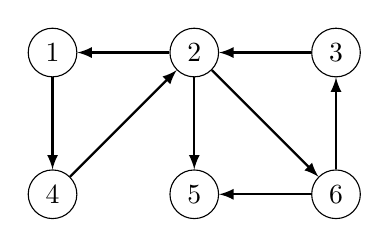
\begin{tikzpicture}[scale=0.9]
\node[draw, circle] (1) at (1,3) {$1$};
\node[draw, circle] (2) at (1,1) {$4$};
\node[draw, circle] (3) at (3,3) {$2$};
\node[draw, circle] (4) at (5,3) {$3$};
\node[draw, circle] (5) at (3,1) {$5$};
\node[draw, circle] (6) at (5,1) {$6$};

\path[draw,thick,->,>=latex] (1) -- (2);
\path[draw,thick,->,>=latex] (2) -- (3);
\path[draw,thick,->,>=latex] (3) -- (1);
\path[draw,thick,->,>=latex] (4) -- (3);
\path[draw,thick,->,>=latex] (3) -- (5);
\path[draw,thick,->,>=latex] (3) -- (6);
\path[draw,thick,->,>=latex] (6) -- (4);
\path[draw,thick,->,>=latex] (6) -- (5);
\end{tikzpicture}
\end{center}
matrica susjedstva je
\[
V= \begin{bmatrix}
  0 & 0 & 0 & 1 & 0 & 0 \\
  1 & 0 & 0 & 0 & 1 & 1 \\
  0 & 1 & 0 & 0 & 0 & 0 \\
  0 & 1 & 0 & 0 & 0 & 0 \\
  0 & 0 & 0 & 0 & 0 & 0 \\
  0 & 0 & 1 & 0 & 1 & 0 \\
 \end{bmatrix}.
\]
Sada, na primjer, matrica
\[
V^4= \begin{bmatrix}
  0 & 0 & 1 & 1 & 1 & 0 \\
  2 & 0 & 0 & 0 & 2 & 2 \\
  0 & 2 & 0 & 0 & 0 & 0 \\
  0 & 2 & 0 & 0 & 0 & 0 \\
  0 & 0 & 0 & 0 & 0 & 0 \\
  0 & 0 & 1 & 1 & 1 & 0 \\
 \end{bmatrix}
\]
sadrži brojeve putova od 4 brida
između čvorova.
Na primjer, $V^4[2,5]=2$,
jer postoje dva puta od 4 brida
od čvora 2 do čvora 5:
$2 \rightarrow 1 \rightarrow 4 \rightarrow 2 \rightarrow 5$
i 
$2 \rightarrow 6 \rightarrow 3 \rightarrow 2 \rightarrow 5$.

\subsubsection{Najkraći putovi}

Koristeći sličnu ideju u težinskom grafu,
možemo za svaki par čvorova izračunati minimalnu
duljinu puta
između njih koji sadrži točno $n$ bridova.
Da bismo to izračunali, moramo definirati množenje matrica
na nov način, tako da ne računamo brojeve
putova, nego minimiziramo duljine putova.

\begin{samepage}
Kao primjer, razmotrimo sljedeći graf:
\begin{center}
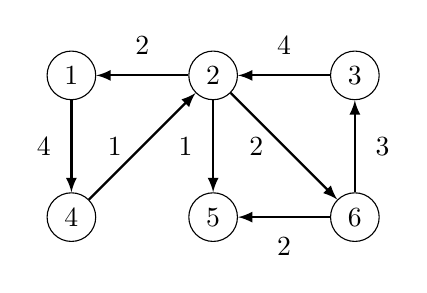
\begin{tikzpicture}[scale=0.9]
\node[draw, circle] (1) at (1,3) {$1$};
\node[draw, circle] (2) at (1,1) {$4$};
\node[draw, circle] (3) at (3,3) {$2$};
\node[draw, circle] (4) at (5,3) {$3$};
\node[draw, circle] (5) at (3,1) {$5$};
\node[draw, circle] (6) at (5,1) {$6$};

\path[draw,thick,->,>=latex] (1) -- node[font=\small,label=left:4] {} (2);
\path[draw,thick,->,>=latex] (2) -- node[font=\small,label=left:1] {} (3);
\path[draw,thick,->,>=latex] (3) -- node[font=\small,label=north:2] {} (1);
\path[draw,thick,->,>=latex] (4) -- node[font=\small,label=north:4] {} (3);
\path[draw,thick,->,>=latex] (3) -- node[font=\small,label=left:1] {} (5);
\path[draw,thick,->,>=latex] (3) -- node[font=\small,label=left:2] {} (6);
\path[draw,thick,->,>=latex] (6) -- node[font=\small,label=right:3] {} (4);
\path[draw,thick,->,>=latex] (6) -- node[font=\small,label=below:2] {} (5);
\end{tikzpicture}
\end{center}
\end{samepage}

Konstruirajmo matricu susjedstva u kojoj
$\infty$ znači da brid ne postoji,
a ostale vrijednosti odgovaraju težinama bridova.
Matrica je
\[
V= \begin{bmatrix}
  \infty & \infty & \infty & 4 & \infty & \infty \\
  2 & \infty & \infty & \infty & 1 & 2 \\
  \infty & 4 & \infty & \infty & \infty & \infty \\
  \infty & 1 & \infty & \infty & \infty & \infty \\
  \infty & \infty & \infty & \infty & \infty & \infty \\
  \infty & \infty & 3 & \infty & 2 & \infty \\
 \end{bmatrix}.
\]

Umjesto formule
\[
AB[i,j] = \sum_{k=1}^n A[i,k] \cdot B[k,j]
\]
sada za množenje matrica koristimo formulu
\[
AB[i,j] = \min_{k=1}^n A[i,k] + B[k,j]
\]
za množenje matrica, pa računamo
minimum umjesto sume,
a zbroj elemenata umjesto umnoška.
Nakon te izmjene
potencije matrice odgovaraju
najkraćim putovima u grafu.

Na primjer, budući da je
\[
V^4= \begin{bmatrix}
  \infty & \infty & 10 & 11 & 9 & \infty \\
  9 & \infty & \infty & \infty & 8 & 9 \\
  \infty & 11 & \infty & \infty & \infty & \infty \\
  \infty & 8 & \infty & \infty & \infty & \infty \\
  \infty & \infty & \infty & \infty & \infty & \infty \\
  \infty & \infty & 12 & 13 & 11 & \infty \\
 \end{bmatrix},
\]
možemo zaključiti da je minimalna duljina puta
od 4 brida
od čvora 2 do čvora 5 jednaka 8.
Takav put je
$2 \rightarrow 1 \rightarrow 4 \rightarrow 2 \rightarrow 5$.

\subsubsection{Kirchhoffov teorem}

\index{Kirchhoffov teorem}
\index{razapinjuće stablo}

\key{Kirchhoffov teorem}
%\footnote{G. R. Kirchhoff (1824--1887) was a German physicist.}
daje način
za računanje broja razapinjućih stabala
grafa kao determinante posebne matrice.
Na primjer, graf
\begin{center}
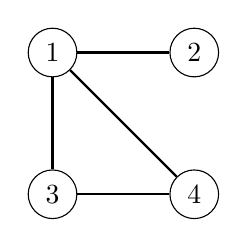
\begin{tikzpicture}[scale=0.9]
\node[draw, circle] (1) at (1,3) {$1$};
\node[draw, circle] (2) at (3,3) {$2$};
\node[draw, circle] (3) at (1,1) {$3$};
\node[draw, circle] (4) at (3,1) {$4$};

\path[draw,thick,-] (1) -- (2);
\path[draw,thick,-] (1) -- (3);
\path[draw,thick,-] (3) -- (4);
\path[draw,thick,-] (1) -- (4);
\end{tikzpicture}
\end{center}
ima tri razapinjuća stabla:
\begin{center}
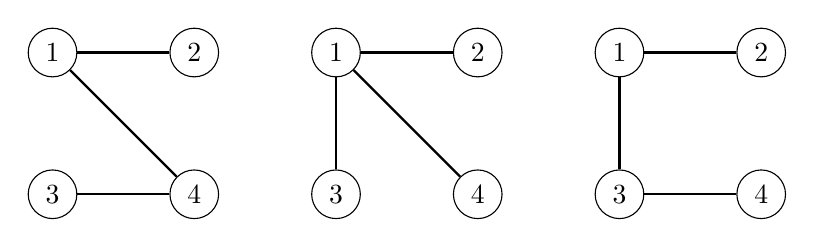
\begin{tikzpicture}[scale=0.9]
\node[draw, circle] (1a) at (1,3) {$1$};
\node[draw, circle] (2a) at (3,3) {$2$};
\node[draw, circle] (3a) at (1,1) {$3$};
\node[draw, circle] (4a) at (3,1) {$4$};

\path[draw,thick,-] (1a) -- (2a);
%\path[draw,thick,-] (1a) -- (3a);
\path[draw,thick,-] (3a) -- (4a);
\path[draw,thick,-] (1a) -- (4a);

\node[draw, circle] (1b) at (1+4,3) {$1$};
\node[draw, circle] (2b) at (3+4,3) {$2$};
\node[draw, circle] (3b) at (1+4,1) {$3$};
\node[draw, circle] (4b) at (3+4,1) {$4$};

\path[draw,thick,-] (1b) -- (2b);
\path[draw,thick,-] (1b) -- (3b);
%\path[draw,thick,-] (3b) -- (4b);
\path[draw,thick,-] (1b) -- (4b);

\node[draw, circle] (1c) at (1+8,3) {$1$};
\node[draw, circle] (2c) at (3+8,3) {$2$};
\node[draw, circle] (3c) at (1+8,1) {$3$};
\node[draw, circle] (4c) at (3+8,1) {$4$};

\path[draw,thick,-] (1c) -- (2c);
\path[draw,thick,-] (1c) -- (3c);
\path[draw,thick,-] (3c) -- (4c);
%\path[draw,thick,-] (1c) -- (4c);
\end{tikzpicture}
\end{center}
\index{Laplaceova matrica}
Za računanje broja razapinjućih stabala
konstruiramo \key{Laplaceovu matricu} $L$,
u kojoj je $L[i,i]$ stupanj čvora $i$,
a $L[i,j]=-1$ ako postoji brid između
čvorova $i$ i $j$, inače je $L[i,j]=0$.
Laplaceova matrica za gornji graf je sljedeća:
\[
L= \begin{bmatrix}
  3 & -1 & -1 & -1 \\
  -1 & 1 & 0 & 0 \\
  -1 & 0 & 2 & -1 \\
  -1 & 0 & -1 & 2 \\
 \end{bmatrix}
\]

Može se pokazati da je
broj razapinjućih stabala jednak
determinanti matrice koja se dobije
kada iz matrice $L$ uklonimo bilo koji redak i bilo koji stupac.
Na primjer, ako uklonimo prvi redak
i prvi stupac, rezultat je

\[ \det(
\begin{bmatrix}
  1 & 0 & 0 \\
  0 & 2 & -1 \\
  0 & -1 & 2 \\
 \end{bmatrix}
) =3.\]
Determinanta je uvijek jednaka,
bez obzira na to koji redak i stupac uklonimo iz matrice $L$.

Uočimo da je Cayleyeva formula iz poglavlja 22.5
poseban slučaj Kirchhoffova teorema,
jer u potpunom grafu s $n$ čvorova vrijedi

\[ \det(
\begin{bmatrix}
  n-1 & -1 & \cdots & -1 \\
  -1 & n-1 & \cdots & -1 \\
  \vdots & \vdots & \ddots & \vdots \\
  -1 & -1 & \cdots & n-1 \\
 \end{bmatrix}
) =n^{n-2}.\]



